\documentclass[12pt,letterpaper]{article}
\usepackage[utf8]{inputenc}
\usepackage[spanish]{babel}
\usepackage{graphicx}
\usepackage[left=2cm,right=2cm,top=2cm,bottom=2cm]{geometry}
\usepackage{graphicx} % figuras
\usepackage{hyperref}
% \usepackage{subfigure} % subfiguras
\usepackage{float} % para usar [H]
\usepackage{amsmath}
%\usepackage{txfonts}
\usepackage{stackrel} 
\usepackage{multirow}
\usepackage{enumerate} % enumerados
\renewcommand{\labelitemi}{$-$}
\renewcommand{\labelitemii}{$\cdot$}
% \author{}
% \title{Caratula}
\begin{document}

% Fancy Header and Footer
% \usepackage{fancyhdr}
% \pagestyle{fancy}
% \cfoot{}
% \rfoot{\thepage}
%

% \usepackage[hidelinks]{hyperref} % CREA HYPERVINCULOS EN INDICE

% \author{}
\title{Caratula}

\begin{titlepage}
\begin{center}
\large{UNIVERSIDAD PRIVADA-DE-TACNA}\\
\vspace*{-0.025in}
\begin{figure}[htb]
\begin{center}

\includegraphics[width=8cm]{./Imagenes/logo}
\end{center}
\end{figure}
\vspace*{0.15in}
INGENIERIA DE SISTEMAS  \\

\vspace*{0.5in}
\begin{large}
TITULO:\\
\end{large}

\vspace*{0.1in}
\begin{Large}
\textbf{INFORME DE LABORATORIO No 01} \\
\end{Large}

\vspace*{0.3in}
\begin{Large}
\textbf{CURSO:} \\
\end{Large}

\vspace*{0.1in}
\begin{large}
INTELIGENCIA DE NEGOCIOS\\
\end{large}

\vspace*{0.3in}
\begin{Large}
\textbf{DOCENTE(ING):} \\
\end{Large}

\vspace*{0.1in}
\begin{large}
 Patrick Cuadros Quiroga\\
\end{large}

\vspace*{0.2in}
\vspace*{0.1in}
\begin{large}
Integrante: \\
\begin{flushleft}
Nilson Felix Laura Atencio	\hfill	(2015053846) 
\end{flushleft}
\end{large}
\end{center}

\end{titlepage}



\thispagestyle{empty} % INDICE SIN NUMERO
\newpage
\setcounter{page}{1} % REINICIAR CONTADOR DE PAGINAS DESPUES DEL INDICE

\section{INFORMACIÓN GENERAL}
	\begin{itemize}
\subsection{Objetivos:}
	\item Conocer los fundamentos sobre Dashboards.
	\item Poder elaborar Dashboard usando Power Bi.
	\item	Utilizar algunas herramientas y funciones de Power Bi
\item	Poder elaborar Dashboard usando Power Bi.

\subsection{Equipos, materiales, programas y recursos utilizados:}
	\item Microsoft SQL Server 2016 o superior
	\item Base de datos AdventureWorks2016 o superior
	\item Power Bi Desktop
	\item Tener una cuenta Microsoft registrada en el Portal de Power Bi
\end{itemize}

\section{MARCO TEORICO}
\begin{itemize}
\subsection{Power Bi:}
	\item Es una solución de análisis empresarial que permite visualizar los datos y compartir información con toda la organización, o insertarla en su aplicación o sitio web. Conéctese a cientos de orígenes de datos y dé vida a sus datos con los paneles e informes dinámicos.
	\item	Power BI es un servicio de análisis empresarial que proporciona información detallada para permitir la toma de decisiones rápidas e informadas.
\item Transforme los datos en impactantes objetos visuales y compártalos con sus colegas en cualquier dispositivo.
\item Explore y analice visualmente los datos, en el entorno local y en la nube, todo en una sola vista.
\item Colabore en paneles personalizados e informes interactivos, y compártalos.
\item Distribúyalos por la organización con un sistema de gobernanza y seguridad integrado

\subsection{Dashboard:}
	\item Es una aplicación que se utiliza para presentar el
contenido de una serie de indicadores que muestran el comportamiento de los datos. 
\item	Un Dashboard, término inglés que se traduce normalmente como panel de instrumentos o salpicadero, es una gráfica que enseña los indicadores fundamentales implicados a la hora de conseguir una serie de objetivos determinados en un negocio. Su uso está orientado a ayudar a la hora de realizar decisiones con las que mejorar la estrategia empresarial, poniendo de manifiesto datos útiles.
\item	Su elaboración es un tema que requiere de especial cuidado, ya que se supone que es una herramienta vital para determinar los pasos a seguir con el fin de hacer crecer una empresa. Lo primero que hay que hacer es determinar cuáles son los indicadores, KPI, correctos y que realmente influyan a la hora de perseguir esos objetivos que se desean superar. Después, se debe hacer especial énfasis en realizar un documento gráfico limpio, claro e informativo, que permita el fácil entendimiento; también ha de permitir que los datos puedan contextualizarse y compararse para realizar valoraciones.
\item	Esta suma de factores hace que cada empresa pueda tener su propio dashboard y que, de hecho, este sea diferente en función de la etapa en la que se encuentre. Evidentemente, no se está en la misma situación cuando se comienza un negocio que, por ejemplo, cuando este lleva una década en activo. De hecho, tampoco se persiguen los mismos objetivos.
\item	Una representación gráfica totalmente fundamental si realmente se quiere hacer crecer una compañía y de la que, a continuación, veremos cuáles son los principales fines con los que se realiza. Su importancia no es baladí.

\end{itemize}
\section{PROCEDIMIENTO}
\begin{itemize}
	\item \textbf{Tarea 1:} Conectar a SQL Server desde Power BI Desktop 


	\item \textbf{Tarea 2:} Adicionar Gráficos al Reporter


	\item \textbf{Tarea 3:} Publicar el reporte en el portal de Power BI
\end{itemize}
\section{ANALISIS E INTERPRETACIÓN DE DATOS}

	\begin{center}
	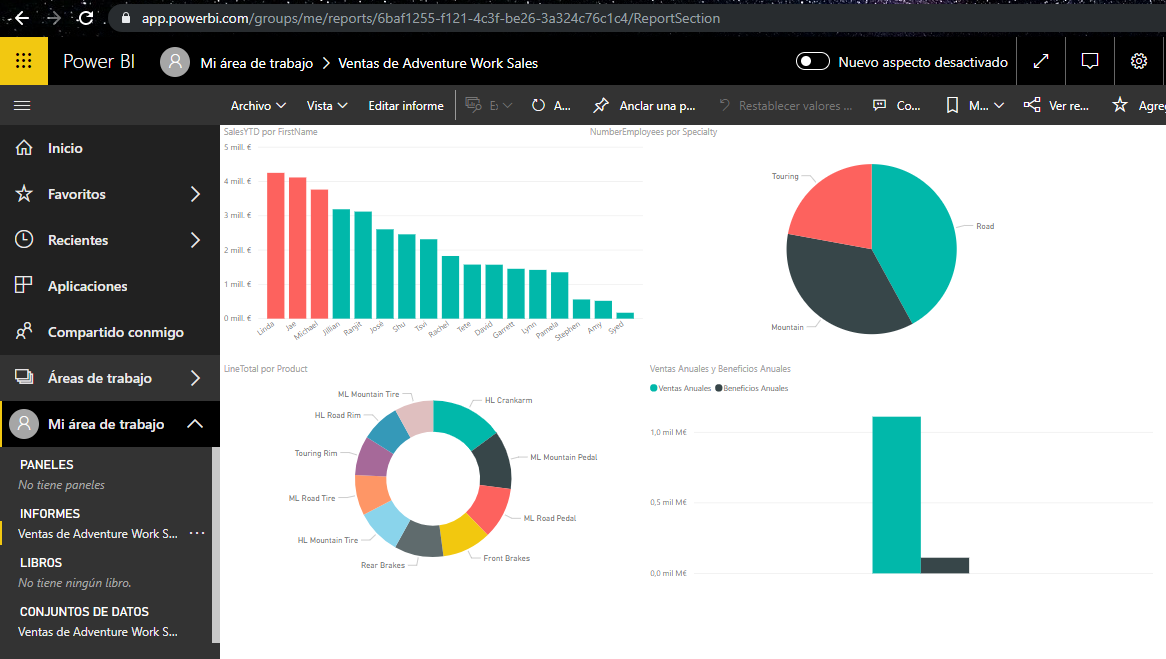
\includegraphics[width=18cm]{./Imagenes/img}
	\end{center}

\section{CONCLUSIONES}
\begin{itemize}
	\item En el desarrollo del laboratorio ha servido para el diseño, implementacion de un dashboard.
	\item Power Bi nos permite un mejor análisis de datos de manera más rápida y sencilla.
\end{itemize}
\section{REFERENCIAS}
\begin{itemize}
	\item Microsoft. ¿Qué es Power BI?. Recuperado de \url{https://powerbi.microsoft.com/es-es/what-is-power-bi/}
	\item Jortilles. Crear un dashboard con Pentaho Bi-Server. Recuperado de \url{http://www.jortilles.com/wp-content/uploads/2016/04/DashboardCDE_Pentaho.pdf}

\end{itemize}


\end{document}
